% \iffalse
\let\negmedspace\undefined
\let\negthickspace\undefined
\documentclass[journal,12pt,twocolumn]{IEEEtran}
\usepackage{cite}
\usepackage{amsmath,amssymb,amsfonts,amsthm}
\usepackage{algorithmic}
\usepackage{graphicx}
\usepackage{textcomp}
\usepackage{xcolor}
\usepackage{txfonts}
\usepackage{listings}
\usepackage{enumitem}
\usepackage{mathtools}
\usepackage{gensymb}
\usepackage{comment}
\usepackage[breaklinks=true]{hyperref}
\usepackage{tkz-euclide} 
\usepackage{listings}
\usepackage{gvv}                                        
\def\inputGnumericTable{}                                
\usepackage[latin1]{inputenc}                            
\usepackage{color}                                       
\usepackage{array}                                       
\usepackage{longtable}                                   
\usepackage{calc}                              
\usepackage{tikz}
\usepackage{multirow}                                    
\usepackage{hhline}                                      
\usepackage{ifthen}                            
\usepackage{caption}
\usepackage{lscape}
\usepackage{amsmath}
\newtheorem{theorem}{Theorem}[section]
\newtheorem{problem}{Problem}
\newtheorem{proposition}{Proposition}[section]
\newtheorem{lemma}{Lemma}[section]
\newtheorem{corollary}[theorem]{Corollary}
\newtheorem{example}{Example}[section]
\newtheorem{definition}[problem]{Definition}
\newcommand{\BEQA}{\begin{eqnarray}}
\newcommand{\EEQA}{\end{eqnarray}}
\newcommand{\define}{\stackrel{\triangle}{=}}
\theoremstyle{remark}
\newtheorem{rem}{Remark}

\begin{document}

\bibliographystyle{IEEEtran}
\vspace{3cm}

\title{NCERT Math 11.9.2 Q8}
\author{EE23BTECH11009 - AROSHISH PRADHAN$^{*}$% <-this % stops a space
}
\maketitle
\newpage
\bigskip
\textbf{Question:} The vertices of $\Delta PQR$ are $P(2, 1)$, $Q(-2, 3)$ and $R(4, 5)$. Find equation of the median through the vertex $R$.\\

\solution
\begin{table}[!h]
    \centering
    \begin{table}[!h]
    \centering
    \begin{tabular}{|c|c|c|}
    \hline
       \textbf{Symbol}  & \textbf{Value} &  \textbf{Description}\\
    \hline
       $V_{in}$  &  &  Input Voltage\\
    \hline
        $V_{out}$ & & Output Voltage\\
    \hline
        $f$ & $1000Hz$ & Input Wave Frequency\\
    \hline
        $T$ & $\dfrac{1}{f} = 10^{-3} s$ & Input Wave Time Period\\
    \hline
        \multirow{4}{*}{$R$} & (a) $0.5k\Omega$ & \multirow{4}{*}{Resistance}\\
        \cline{2-2}
        & (b) $5k\Omega$ &\\
        \cline{2-2}
        & (c) $0.5k\Omega$ &\\
        \cline{2-2}
        & (d) $5k\Omega$ &\\
    \hline
        \multirow{4}{*}{$C$} & (a) $0.1\mu F$ & \multirow{4}{*}{Capacitance}\\
        \cline{2-2}
        & (b) $1\mu F$ &\\
        \cline{2-2}
        & (c) $0.1\mu F$ &\\
        \cline{2-2}
        & (d) $1\mu F$ &\\
    \hline
        $\tau$ & $RC$ & Time Constant\\
    \hline
    \end{tabular}
    \caption{Given Parameters}
    \label{tab:1_gate.23.ph.37}
\end{table}

    \caption{Given Parameters}
    \label{tab:1}
\end{table}
\begin{figure}[!h]
    \centering
    \begin{tikzpicture}
  \coordinate (P) at (2, 1);
  \fill (P) circle (2pt);
  \coordinate (Q) at (-2, 3);
  \fill (Q) circle (2pt);
  \coordinate (R) at (4, 5);
  \fill (R) circle (2pt);

  \draw (P) -- (Q) -- (R) -- cycle;
  \coordinate (M) at ($(P)!0.5!(Q)$);

  \draw[dashed] (R) -- (M);  
  \node[below] at (P) {$P(2, 1)$};
  \node[above left] at (Q) {$Q(-2, 3)$};
  \node[above right] at (R) {$R(4, 5)$};
  \fill (M) circle (2pt) node[below left]{$M(0, 2)$};
\end{tikzpicture}

    \caption{$\Delta PQR$}
    \label{fig:1}
\end{figure}

Coordinates of mid-point $M$ of $PQ$ are given by:
\begin{align}
    (x_M, y_M) &= \left(\dfrac{x_P + x_Q}{2}, \dfrac{y_P + y_Q}{2}\right)\\
    &= (0, 2)
\end{align}
$\therefore$ equation of median $RM$:
\begin{align}
    y-2 &= \left(\dfrac{5-2}{4-0}\right)(x-0)\\
    \implies y &= \dfrac{3}{4} x + 2
\end{align}
\begin{enumerate}
\item Plotting the discrete signal:
    \begin{equation}
        x(n) = \left(\dfrac{3}{4} n + 2\right) u(n)
    \end{equation}
    where,
    \begin{equation}
        u(n) = \begin{cases}
                    0 & :n<0\\
                    1 & :n \geq 0
               \end{cases}
    \end{equation}
    \begin{figure}[!h]
        \centering
        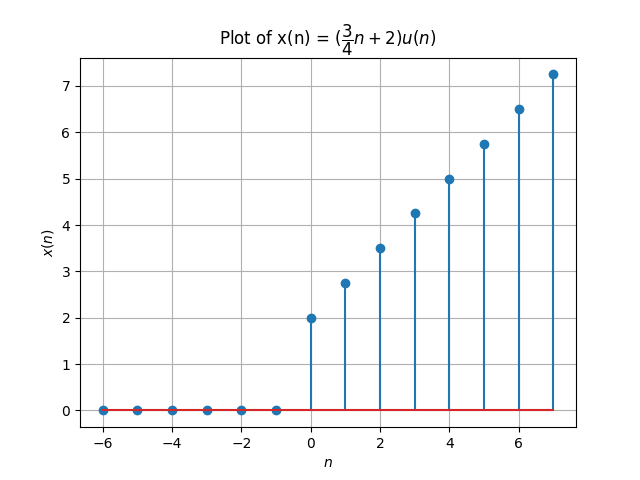
\includegraphics[width = \columnwidth]{figs/fig2.png}
        \caption{Plot of x(n)}
        \label{fig:2}
    \end{figure}
\item Z-Transform of $x(n)$
    \begin{align}
        x(n) &\overset{z}{\longleftrightarrow} X(z)\\  
        \implies X(z) &= \mathcal{Z}\{x(n)\} = \sum_{n=-\infty}^{\infty} x(n)z^{-n}\\
        &= \sum_{n=-\infty}^{\infty} \left(\frac{3}{4}n + 2\right)u(n)z^{-n}\\
        &= \frac{3}{4}\sum_{n=0}^{\infty}nz^{-n} + 2 \sum_{n=0}^{\infty}z^{-n}\\
        &= \frac{3}{4}S_2 + 2 S_1\label{eq:11}
    \end{align}
    Solving the summations:
    \begin{enumerate}
        \item $S_1$
            \begin{align}
                S_1 &= \sum_{n=0}^{\infty} z^{-n}\label{eq:12}\\
                &= \dfrac{1}{1-z^{-1}}\label{eq:13}
            \end{align}
        \item $S_2$
        
            From \eqref{eq:12} and \eqref{eq:13},
            \begin{align}
                \sum_{n=0}^{\infty} z^{-n} &= \dfrac{1}{1-z^{-1}}\\
                \implies \dfrac{d}{dz}\left(\sum_{n=0}^{\infty} z^{-n}\right) &= \dfrac{d}{dz}\left(\dfrac{1}{1-z^{-1}}\right)\\
                \implies \sum_{n=0}^{\infty} -n z^{-n-1} &= \dfrac{-z^{-2}}{1-z^{-1}}\\
                \implies S_2 = \sum_{n=0}^{\infty} n z^{-n} &= \dfrac{z^{-1}}{(1-z^{-1})^2}\label{eq:16}
            \end{align}
    \end{enumerate}
    Using \eqref{eq:13} and \eqref{eq:16} in \eqref{eq:11}
    \begin{align}
        X(z) = \dfrac{3}{4}\dfrac{z^{-1}}{(1-z^{-1})^2} + \dfrac{2}{1-z^{-1}}
    \end{align}
    where $\{z\in \mathbb{C} : \abs{z} > 1 \}$
\end{enumerate}
\end{document}
